%%%%%%%%%%%%%%%%%%%%%%%%%%%%%%%%%%
% EL/EEE D1 Report Template
% University of Southampton
%
% author : Rhys Thomas (rt8g15)
%
% edited : 2016-11-14
%%%%%%%%%%%%%%%%%%%%%%%%%%%%%%%%%%

\documentclass[a4paper,11pt]{article}

%%%%%%%%%%%%%%%%%%%%%%%%%%%%%%%%%%
% PACKAGES
%%%%%%%%%%%%%%%%%%%%%%%%%%%%%%%%%%
\usepackage[margin=1in]{geometry}
\renewcommand{\baselinestretch}{1.2} % line spacing
\usepackage{color}
\usepackage{siunitx}
\usepackage{graphicx}
\usepackage{epstopdf}
\usepackage{float}
\usepackage{hyperref}
\usepackage{mathtools}
\usepackage[titletoc,toc,title]{appendix}
\usepackage{subfiles}
\usepackage{pgfplots}
\usepackage[european]{circuitikz}
\usepackage{textgreek}
\usepackage{amssymb}
\usepackage{subfig}

\pgfplotsset{compat=1.13}
\pgfplotsset{unit code/.code={\si{#1}}}
\usepgfplotslibrary{units}

\graphicspath{ {./images/} }

\usepackage{newunicodechar}
\newunicodechar{p}{\ifmmode\pi\else\textpi\fi}

%%%%%%%%%%%%%%%%%%%%%%%%%%%%%%%%%%
% DOCUMENT BEGIN
%%%%%%%%%%%%%%%%%%%%%%%%%%%%%%%%%%
\begin{document}
  
\begin{center}
{\Large{\textbf{ELEC2205 D3 -- Two-Stage Amplifier Design}}} \\ [\baselineskip]
\subfile{info.tex}
\end{center}

\begin{abstract}
\end{abstract}

\tableofcontents
\newpage

\section{Theoretical Design}
\subsection{Voltage Gain Derivation}
\subsubsection{Stage 1}

\begin{figure}[h]
\centering
    \subfile{./circuits/stage1Circuit.tex}
    \caption{Circuit diagram of the first stage of the amplifier.}
    \label{fig:stage1}
\end{figure}

In order to derive the voltage gain of this circuit, we need to analyse it using a small signal model. The hybrid-\textpi\ model (figure~\ref{fig:stage1hpi}) will be used.

\begin{figure}[h]
\centering
    \subfile{./circuits/stage1hpi.tex}
    \caption{Hybrid-\textpi\ model of the first stage of the amplifier.}
    \label{fig:stage1hpi}
\end{figure}

Using Kirchoff's current law on the base:

\begin{subequations}
\begin{align}
\frac{v_b - v_s}{R_s} + \frac{v_b}{R_2} + \frac{v_b}{R_1} + \frac{v_b - v_e}{r_\pi} &= 0\\
\frac{v_b - v_s}{R_s} + v_b \left(\frac{1}{R_1} + \frac{1}{R_2} \right) + \frac{v_b - v_e}{r_\pi} &= 0 \label{eq:kclBase}
\end{align}
\end{subequations}

It can be seen that $v_\pi = v_b - v_e$. The small signal output resistance, $r_\pi$, is defined as $\frac{\beta}{g_m}$~\cite[p. 29]{ADAIC}.

Using Kirchoff's current law on the emitter:

\begin{subequations}
\begin{align}
&\frac{v_e - v_b}{r_\pi} - g_m (v_b - v_e) + \frac{v_e}{R_{e2}} + \frac{v_e - v_c}{r_0} = 0\\
\textrm{Assuming $r_0$ is large: } &\frac{v_e - v_b}{r_\pi} - g_m (v_b - v_e) + \frac{v_e}{R_{e2}} = 0 \label{eq:kclEmitter}
\end{align}
\end{subequations}

Using Kirchoff's current law on the collector:

\begin{equation} \label{eq:kclCollector}
\frac{v_c}{R_c} + g_m(v_b - v_e) = 0
\end{equation}

Substituting the definition of $r_\pi$ into equation~\ref{eq:kclEmitter}:

\begin{subequations}
\begin{align}
\frac{(v_e - v_b)g_m}{\beta} - g_m(v_b - v_e) + \frac{v_e}{R_{e2}} &= 0\\
g_m \left( \frac{v_e - v_b}{\beta} + (v_e - v_b) \right) + \frac{v_e}{R_{e2}} &= 0\\
g_m (v_e - v_b) \left( \frac{1}{\beta} + 1 \right) + \frac{v_e}{R_{e2}} &= 0 \label{eq:kclEmitter2}
\end{align}
\end{subequations}

Equating equations \ref{eq:kclEmitter2} and \ref{eq:kclCollector}:

\begin{subequations}
\begin{align}
g_m (v_e - v_b) \left( \frac{1}{\beta} + 1 \right) + \frac{v_e}{R_{e2}} &= \frac{v_c}{R_c} + g_m(v_b - v_e)\\
g_m (v_e - v_b) \left( \frac{1}{\beta} + 2 \right) + \frac{v_e}{R_{e2}} &= \frac{v_c}{R_c} \label{eq:emitterEqCollector}
\end{align}
\end{subequations}

By Ohm's law:

\begin{subequations}
\begin{align}
v_e &= i_e R_{e2}\\
&= R_{e2} (i_b + i_c)\\
&= R_{e2} (i_b + \beta i_b)\\
&= R_{e2} i_b (\beta + 1) \label{eq:v_e}
\end{align}
\end{subequations}

\begin{subequations}
\begin{align}
v_b - v_e &= r_\pi i_b\\
\therefore v_b - R_{e2} i_b (\beta + 1) &= r_\pi i_b
\end{align}
\end{subequations}

\begin{subequations}
\begin{align}
v_c &= -i_c R_c\\
&= -\beta i_b R_c \label{eq:v_c}
\end{align}
\end{subequations}

Substituting equation \ref{eq:v_e} into \ref{eq:emitterEqCollector}

\begin{subequations}
\begin{align}
g_m \left(R_{e2} i_b (\beta + 1) - v_b\right) \left( \frac{1}{\beta} + 2 \right) + i_b (\beta + 1) &= \frac{v_c}{R_c}
\end{align}
\end{subequations}

\newpage
\section{Voltage Gain Measurement}
    The voltage gain of each stage of the amplifier was measured by supplying an alternating voltage at the input, and measuring the amplitude of the voltage at the output. The gain of both stages combined was also measured this way. The measurements are shown in figure~\ref{fig:oscgain} and consolidated in table~\ref{tab:gain}.
    
        \begin{figure}[h]
            \centering
            \subfloat[Oscilloscope captures of input and output signals][Stage 1]
            {
                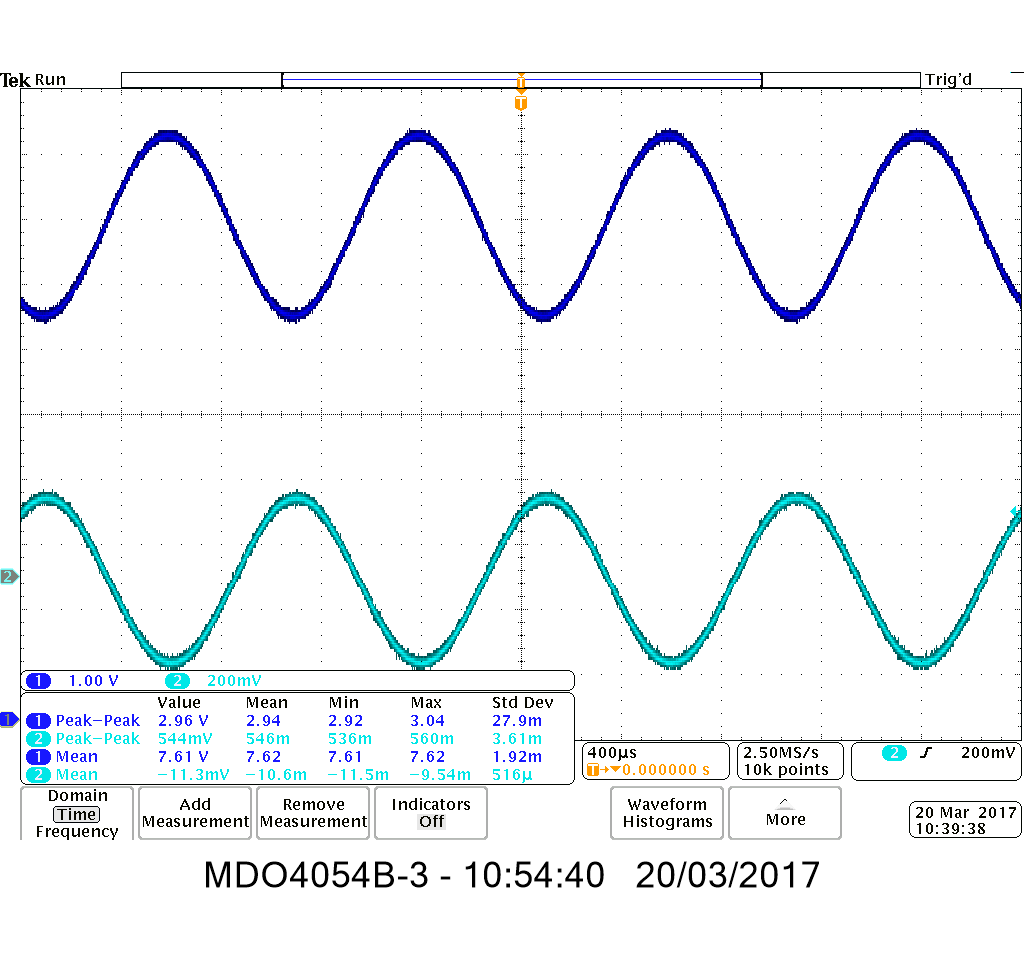
\includegraphics[width = 0.45\textwidth]{stage1gain.png}
                \label{fig:oscgain1}
            }
            \subfloat[Oscilloscope captures of input and output signals][Stage 2]
            {
                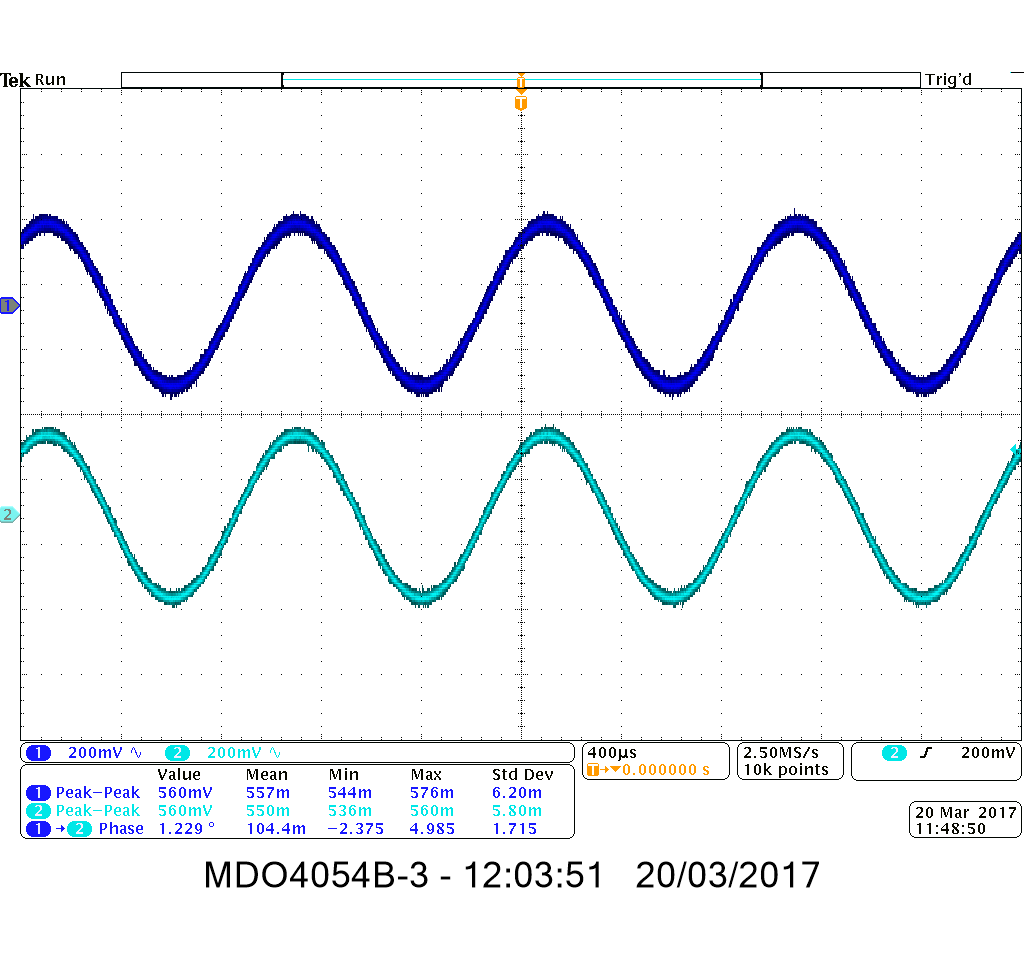
\includegraphics[width = 0.45\textwidth]{stage2gain.png}
                \label{fig:oscgain2}
            }
            \qquad
            \subfloat[Oscilloscope captures of input and output signals][Combined]
            {
                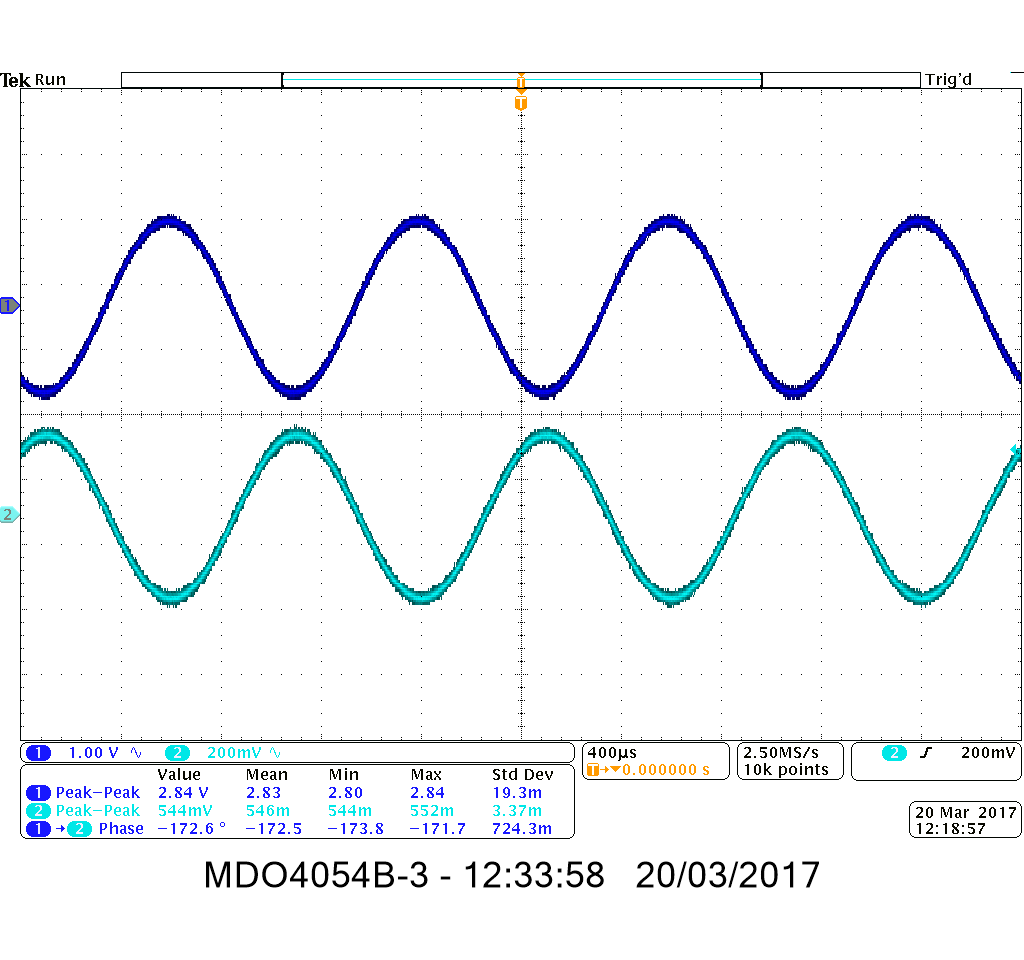
\includegraphics[width = 0.4\textwidth]{totalgain.png}
                \label{fig:oscgaintot}
            }
            \caption{Oscilloscope captures of input and output signals. The top waveform (2) in each image is the output, and the bottom (1) is the output.}
            \label{fig:oscgain}
        \end{figure}
    
        \begin{table}[h]
            \centering
            \subfloat[][Stage 1]
            {
                \begin{tabular}{|l|l|}
                    \hline
                    \textbf{Frequency}      & \SI{1}{\kilo\hertz}           \\ \hline
                    \textbf{Input Voltage}  & \SI{500}{\milli\volt_{pp}}    \\ \hline
                    \textbf{Output Voltage} & \SI{2.96}{\volt_{pp}}         \\ \hline
                    \textbf{Gain}           & 5.92                          \\ \hline
                \end{tabular}
                \label{tab:s1gain}
            }
            \subfloat[][Stage 2]
            {
                \begin{tabular}{|l|l|}
                    \hline
                    \textbf{Frequency}      & \SI{1}{\kilo\hertz}           \\ \hline
                    \textbf{Input Voltage}  & \SI{500}{\milli\volt_{pp}}    \\ \hline
                    \textbf{Output Voltage} & \SI{558}{\milli\volt_{pp}}    \\ \hline
                    \textbf{Gain}           & 1.01                          \\ \hline
                \end{tabular}
                \label{tab:s2gain}
            }
            \qquad
            \subfloat[][Combined]
            {
                \begin{tabular}{|l|l|}
                    \hline
                    \textbf{Frequency}      & \SI{1}{\kilo\hertz}           \\ \hline
                    \textbf{Input Voltage}  & \SI{500}{\milli\volt_{pp}}    \\ \hline
                    \textbf{Output Voltage} & \SI{2.83}{\volt_{pp}}         \\ \hline
                    \textbf{Gain}           & 5.66                          \\ \hline
                \end{tabular}
                \label{tab:scombgain}
            }
            \caption{Tables of measurements made from the two amplifier stages, and the amplifier with both stages combined.}
            \label{tab:gain}
        \end{table}

\newpage
\section{Impedance Measurement}
    Impedance values were calculated by measuring the voltage across a resistor with a value estimated to be near the actual impedance.
    
    \subsection{Stage 1}
        \subsubsection{Input impedance}
            \begin{figure}[h]
            \centering
                \subfile{./circuits/stage1InputImpedance.tex}
                \caption{Measuring the input impedance of the first amplification stage.}
                \label{fig:stage1inputZ}
            \end{figure}
            
            \begin{subequations} \label{eq:stage1Rin}
            \begin{align}
                \frac{V_{i1}}{V_{i1}'} &= \frac{R_{in1}}{R_{in1} + 47000}   \\
                \frac{79.2}{177} &= \frac{R_{in1}}{R_{in1} + 47000}   \\
                \therefore R_{in1} &= \SI{45.1}{\kilo\ohm}
            \end{align}
            \end{subequations}
            
            As shown by equation set~\ref{eq:stage1Rin}, the input impedance of stage 1 was calulated to be \SI{45.1}{\kilo\ohm}.
        
        \subsubsection{Output impedance}
        
            \begin{figure}[h]
            \centering
                \subfile{./circuits/stage1OutputImpedance.tex}
                \caption{Measuring the output impedance of the first amplification stage.}
                \label{fig:stage1outputZ}
            \end{figure}
            
            \begin{subequations} \label{eq:stage1Rout}
            \begin{align}
                \frac{V_{o1}}{V_{o1}'} &= \frac{R_{out1}}{R_{out1} + 47000}   \\
                \frac{265}{530} &= \frac{R_{out1}}{R_{out1} + 47000}   \\
                \therefore R_{out1} &= \SI{1.8}{\kilo\ohm}
            \end{align}
            \end{subequations}
            
            As shown by equation set~\ref{eq:stage1Rout}, the output impedance of stage 1 was calulated to be \SI{1.8}{\kilo\ohm}.
        
    \subsection{Stage 2}
        \subsubsection{Input impedance}
            \begin{figure}[h]
            \centering
                \subfile{./circuits/stage2InputImpedance.tex}
                \caption{Measuring the input impedance of the second amplification stage.}
                \label{fig:stage2inputZ}
            \end{figure}
            
            \begin{subequations} \label{eq:stage2Rin}
            \begin{align}
                \frac{V_{i2}}{V_{i2}'} &= \frac{R_{in2}}{R_{in2} + 27000}   \\
                \frac{111}{177} &= \frac{R_{in2}}{R_{in2} + 27000}   \\
                \therefore R_{in2} &= \SI{45.4}{\kilo\ohm}
            \end{align}
            \end{subequations}
            
            As shown by equation set~\ref{eq:stage2Rin}, the input impedance of stage 2 was calulated to be \SI{45.4}{\kilo\ohm}.
    
        \subsubsection{Output impedance}
            \begin{figure}[h]
            \centering
                \subfile{./circuits/stage2OutputImpedance.tex}
                \caption{Measuring the output impedance of the second amplification stage.}
                \label{fig:stage2outputZ}
            \end{figure}
            
            \begin{subequations} \label{eq:stage2Rout}
            \begin{align}
                \frac{V_{o2}}{V_{o2}'} &= \frac{R_{out2}}{R_{out2} + 68}   \\
                \frac{66}{178} &= \frac{R_{out2}}{R_{out2} + 68}   \\
                \therefore R_{out2} &= \SI{40.1}{\ohm}
            \end{align}
            \end{subequations}
            
            As shown by equation set~\ref{eq:stage2Rout}, the output impedance of stage 2 was calulated to be \SI{40.1}{\ohm}.
            
    \subsection{Combined}
        \subsubsection{Input impedance}
            This was measured using the same method as when measuring the input impedance of the first stage alone.
            
            \begin{subequations} \label{eq:Rin}
            \begin{align}
                \frac{V_{i}}{V_{i}'} &= \frac{R_{in}}{R_{in} + 47000}   \\
                \frac{86.2}{177} &= \frac{R_{in}}{R_{in} + 47000}   \\
                \therefore R_{in} &= \SI{44.6}{\kilo\ohm}
            \end{align}
            \end{subequations}
            
            As shown by equation set~\ref{eq:Rin}, the input impedance of the combined amplifier was calulated to be \SI{44.6}{\kilo\ohm}.
            
        \subsubsection{Output impedance}
            This was measured using the same method as when measuring the output impedance of the second stage alone.
            
            \begin{subequations} \label{eq:Rout}
            \begin{align}
                \frac{V_{o}}{V_{o}'} &= \frac{R_{in}}{R_{out} + 68}   \\
                \frac{147}{929} &= \frac{R_{out}}{R_{out} + 68}   \\
                \therefore R_{out} &= \SI{12.8}{\ohm}
            \end{align}
            \end{subequations}
            
            As shown by equation set~\ref{eq:Rout}, the output impedance of the combined amplifier was calulated to be \SI{12.8}{\ohm}.

\newpage
\section{Reflection or w/e}

\newpage
\begin{appendices}
    \label{appendix}
    \section{Some appendix}
    \label{app:one}
\end{appendices}

\bibliographystyle{IEEEtran}
% IEEEabrv abbreviates journal titles in accordance to IEEE standards 
\bibliography{mybib}

\end{document}